
\chapter{Complexity Classes and Relevance of the Problem}
\epigraph{“Either mathematics is too big for the human mind or the human mind is more than a machine.” }{\textit{Kurt Godël\cite{goldblatt2014topoi}}}
\section{Model of Computation}


Computation started as a way of relieving mathematicians of mechanical work. A long journey has been made by now. In particular, models of computation improve our ability to ease work to unexpected limits. Nonetheless some barriers are still left to breaks. In particular there is the dream of a efficient theorem prover, that will made mathematicians life easier, so that formalism would be relegated to the domain of machines, just as arithmetic has already been done.The work of the mathematician would then be to check and understand what things are important and how to pose the problems in the right language.\\

SAT, and even more QBF, try to solve this problem, by asserting veracity of simple laws. Some projects such as COQ\cite{bertot2008short} have been doing work on this area. They have had limited success, because of the complexity of the problem  we have before us. In this chapter we present the theory of complexity and the state of the art of the complexity analysis. We reflex upon the P vs NP problem and we present sat as the cornerstone for the development of this theory, having as its zenith the Cook-Levin Theorem [\ref{ref:cooklevin}].

\subsection{Deterministic Computation}
In this section we discuss two computation models: Turing Machines and Circuits. We do not expect the text to be the first approximations to Turing machines, so we present a quick formal approach to the area.  \\

Turing machines are arguably the epicenter of  models of computation. A Turing Machine  represents a long mechanical tape on which we are going to operate. The tape is divided into discrete positions, such that we can see the tape as a one-dimensional array. Operating on this tape we can focus on a cell, scan its contents, overwrite  its contents or move to an adjacent cell. These operations try to resemble the process of human calculus, as done with paper and pencil when applying the long division method  for example. Formally:

\begin{definition}[Turing Machine \cite{hopcroft2007introduction}] We describe a Turing Machine as a 7-tuple $M=(Q, \Sigma, \Gamma, \delta, q_0, B, F)$ whose components have the following meanings:
  \begin{itemize}
  \item $Q$ the finite set of \emph{states} of the finite control.
  \item $\Sigma$ the finite set of \emph{input symbols}.
  \item $\Gamma$ the finite set of \emph{tape symbols}. $\Sigma$ is always a subset of $\Gamma$.
  \item  $\delta: Q\times \Gamma \to Q\times\Gamma\times\{L,R\}$ the transition function.
  \item $q_0$ the \emph{start state}.
  \item $B$ the \emph{blank symbol}.
  \item $F$ the \emph{accepting states}.
  \end{itemize}

  A configuration of a Turing machine is a triplet $C=(q,u,v)$ where $q\in Q$, $u,v\in \Gamma^*$. A configuration is accepting if $q\in F$.
\end{definition}

A configuration should be understand as a state of the machine, where $q$ is the current state, $u$ the part of the tape left to the cell on which we focus and $v$ is the part of the tape right to the cell we focus, starting on it.\\

As a brief note before going on, we have not defined the empty word yet, as in propositional logic is not a valid formula so it lacks our interest until now. We will note the empty word as $\epsilon$ and would consist of an empty sequence of symbols. We can  now define a relation between configurations:

\begin{definition}\label{def:paso}
  Let $M$ be a Turing Machine (TM) and $C=(q,u,v)$, $C'=(q,u,v)$ be two configurations of $M$. We say that $C\vdash C'$ if there is a transition $\delta (q,v_1) = (q', b, D) $ with $D\in{L,R}$ and:
  \begin{itemize}
  \item if $D=L$, then if $u=u_1...u_n$ and $v = v_1...v_m$, it should happen that $u' = u_1...u_{n-1}$ and $v' = u_n bv_2...v_n$ with two exceptions:
    \begin{itemize}
    \item if $u=\epsilon$ then $u' = \epsilon$ and $v' = bv_2...v_n,$
    \item if $v = v_1$ and $b =B$ then $u'=u_1...u_{n-1}$ and $v' = u_n$.
    \end{itemize}

  \item if $D=R$, then if $u=u_1...u_n$ and $v = v_1...v_m$, it should happen that $u' = u_1...u_{n}b$ and $v' = v_2...v_n$ with two exceptions:
    \begin{itemize}
    \item if $u=\epsilon$ then $u' = b$ and $v' =v_2...v_n,$
    \item if $v = v_1$ and $b =B$ then $u'=u_1...u_{n-1}$ and $v' = \epsilon$.
    \end{itemize}
  \end{itemize}

  Note that on both cases the two exceptions can be given simultaneously. We say $C\vdash^* C'$ if there exists a finite sequence $\{C_i\}_{i\in 1,...,n}$ such that $C_1 = C$, $C_n=C'$ and $C_i\vdash C_{i+1}$ for every $i\in 1,...,n-1$.  
  \end{definition}

  When it is beneficial we can consider a TM $M$ to have an output, that is, to explicitly say whether or not $M$ accepts a word.\\

  
  We now describe the use of Turing Machine: solving problems. We consider that Turing Machines solve both decision and function problems. Lets start by explaining how a Turing Machine solves a decision problem.

  \begin{definition}
     Let $M$ be a Turing Machine. We say that $u\in\Sigma^*$ is \emph{accepted} by $M$ if there exists a final configuration $C$ such that $(q_0,\epsilon,u)\vdash^* C$. The language \emph{accepted} by $M$ denoted as $L(M)$ is the collection of all words accepted. We say that $M$ \emph{decides} a language $L$ if $L$ is the language accepted by $M$.
  \end{definition}

  With regard to solving a function problem, the intuitive idea is that we write the input on the tape and after some computations we have written on the tape a word that is related to the input one. Formally:


  \begin{definition}
    Let $R\subset\Sigma^*\times \Sigma^*$ be a relation. A Turing Machine $M$ \emph{compute} $R$ if for every $u\in \Sigma^*$ there is an accepting configuration $C=(q',v,v')$ of $M$  such that $(q,\epsilon,u)\vdash^* C$ and $(u,vv') \in R$. A Turing Machine $M$ computes a function problem defined by $R$ if it computes $R$.
  \end{definition}


%  Among the turing machines, the universal turing machine should be highlighted.It was Turing who elucidated that a turing machine could be built such that by giving as an input the description of a Turing machine and a word would act as the described machine when receiving that word as input.
  

  \subsection{Non-deterministic Computation}
Analogous to the concept of Turing Machine, another recurrent idea in computation is the concept of non-deterministic computing. These models allow an algorithm to react different to the same input. These models are useful as there as they encapsulate various problem of interest and give upper bound to the deterministic complexity. In order to formalize this concept we will define non-deterministic Turing Machines.\\

Intuitively, a non-deterministic Turing Machine is a Turing Machine that, at any point on its computation, can choose from several different 'paths' to compute. This choice is made in a non-deterministic manner, that is, it is not known what the result will be until the computation is done.

\begin{definition}\label{def:NDTM} We describe a Non-Deterministic Turing Machine (NDTM) as a 7-tuple $M=(Q, \Sigma, \Gamma, \delta, q_0, B, F)$ whose components have the following meanings:
  \begin{itemize}
  \item $Q$ the finite set of \emph{states} of the finite control.
  \item $\Sigma$ the finite set of \emph{input symbols}.
  \item $\Gamma$ the finite set of \emph{tape symbols}. $\Sigma$ is always a subset of $\Gamma$.
  \item  $\delta\subset (Q\times \Gamma)\times( Q\times\Gamma\times\{L,R\})$ the transition relation.
  \item $q_0$ the \emph{start state}.
  \item $B$ the \emph{blank symbol}.
  \item $F$ the \emph{accepting states}.
  \end{itemize}

  A configuration of a Turing machine is a triplet $C=(q,u,v)$ where $q\in Q$, $u,v\in \Gamma^*$. A configuration is accepting if $q\in F$.
\end{definition}

Note that there exists $d_0 \in \mathbb{N}$ such that:
  $$ \left| \left \{ (q,\gamma',D) \in  ( Q\times\Gamma\times\{L,R\})\ :\ ( (p,\gamma), (q,\gamma',D) ) \in \delta \right \}\right | \le d_0.$$
  Such $d_0$ is called \emph{branching factor} of $M$.\\

By opposition, the previously defined Turing machines are considered Deterministic Turing Machines(DTM). The definition of Non-Deterministic Turing Machine is adapted from \cite{hopcroft2007introduction}. \\
  
The definition [\ref{def:paso}] holds for non-deterministic Turing machines, with the consideration that now instead of finding the image of a function we have to find a related triple. Using analogous notions we define when a problem is decided/computed by a Non-deterministic Turing Machine. A Non-Deterministic Turing machine can be regarded as a tree. In this tree we assume that a branch divides when a decision has to be made. Once this tree is built, we can assume that the execution of our TM will be the progression of one of the possible paths of the tree.\\


  
\subsection{Reductions}

Once we now how to make a TM for one problem, we may ask ourselves: can we make a TM machine in order to solve more that one problem?. To answer this question we define the notion of reduction. Intuitively, a reduction is a process in which, instead of solving two problem $L_1$ and $L_2$, we choose to only solve $L_1$ and use its resolution in order to solve $L_2$. Formally:

\begin{definition}
If $L_1$ and $L_2$ are decision problems, then we say that $L_1$ is reduced to $L_2$ is there is an TM that always stops and computes a function $f$ such that for every input $w$ to $L_1$ , we have that $L_2$ produces the same answer for the input $f (w )$.  
\end{definition}


This notion also provides us with a partial order relationship. For function problem we can state the analogue definition. 


\section{Complexity Classes}
\label{sec:complexity}

In this section we are going to define what a complexity class is and then we are going to discuss some results of the complexity of the SAT-problem. We use as principal reference \cite{arora2009computational}.

\subsection{Deterministic complexity}
\label{sub:detcomp}
There are different approaches as how to measure the complexity of given algorithm. We will focus primarily on \emph{worst-case time complexity}. We will also introduce \emph{worst-case space complexity} and provide some results.

\begin{definition}
  Let $g:\mathbb{N}^\mathbb{N}$, the:
  $$O(g) = \left\{ f\in \mathbb{N}^\mathbb{N} :\ \exists N,C \in \mathbb{N} : f(n) \le Cg(n) \ \forall  n \ge N\right\}.$$
\end{definition}

\begin{definition}
  Let $f:\mathbb{N}^\mathbb{N}$.
\begin{enumerate}
  \item We let \emph{TIME}$(f)$ (resp. \emph{FTIME}$(f)$) be the set of all decision  problems (resp. function problems) that can be decided (resp. computed) by a Turing machine $M$ using less that $g(n)$ steps where $g\in O(f)$ and $n$ is the number of characters of the input.  
  \item We let \emph{SPACE}$(f)$ (resp. \emph{FSPACE}$(f)$) be the set of all decision problems (resp. function problems) that can be decided (resp. computed) by a Turing machine $M$ using less that $g(n)$ cells where $g\in O(f)$ and $n$ is the number of characters of the input.  
  \end{enumerate}

\end{definition}

Sometimes we will also consider the TM $M$ that decides/computes the problem to be in $TIME(f)$ if the context is clear enough. This definition let us a great tool in order to define collections of problems, and to compare them. We introduce some classes.
\begin{definition}
  Let $\Omega$ be a set of endofunctions of $\mathbb{N}$.
  \begin{enumerate}
  \item We have a homonym complexity class $\Omega$:
  $$\Omega =  \bigcup_{f \in \Omega} TIME(f). $$
  \item We have an associated function complexity class $FA$:
    $$F\Omega =  \bigcup_{f \in \Omega} FTIME(f).$$
  \item We have an associated space complexity class $FA$:
    $$\Omega SPACE =  \bigcup_{f \in \Omega} SPACE(f).$$  \end{enumerate}
\end{definition}


Although we have define the complexity classes as collections of decision problems, we can also consider consider a language to be in a class $C$ if its associated decision problem is. During the study we will focus on decision problem complexity classes. Nonetheless ties between this classes and its associated function complexity classes are strong and will be pointed out.\\

In general the notation of complexity classes is additive. Therefore is we want to represent the function space complexity class associated to $\Omega$ we denote that by $F\Omega SPACE$.\\


Arguably the most important of the complexity classes is P. We define P as the set of all polynomials. Therefore we have an homonym complexity class P. We can justify the importance of this class the Feasibility Thesis.

\begin{thesis}[\cite{cook2006p}]
A natural problem has a feasible algorithm iff it has a polynomial-time algorithm.
\end{thesis}

That is, only problems with polynomial time complexity are able to be computed, as otherwise their complexity make them not viable, i.e., not computable in a coherent time. The idea of problems being not feasible is the basis of some of the most important conceptions of modern Computer Science. In particular in modern cryptoanalysis the most common encoding technique (private keys protocols) are based upon the conception that no one would be able to solve the presented problem without some added information in a coherent time, independently of their computing capabilities.\\

Other important class on complexity is L. We define L as the set of all Linear combination of logarithms. Now we need to point out that in most part of literature, the class L refer to the class we named LSPACE. Nonetheless we decide to maintain out notation for internal coherence of the text. 

\subsection{Non-Deterministic Complexity}

As with TM we can consider complexity classes based on non-deterministic procedures.

\begin{definition}
  Let $f: \mathbb{N}\to  \mathbb{N}$.
\begin{enumerate}
  \item We let \emph{NTIME}$(f)$  the set of all problems that can be decided/computed by a non-deterministic Turing machine $M$ using less that $g(n)$ steps where $g\in O(f)$ and $n$ is the number of characters of the input.  
  \item We let \emph{NSPACE}$(f)$  the set of all problems that can be decided/computed by a non-deterministic Turing machine $M$ using less that $g(n)$ cells where $g\in O(f)$ and $n$ is the number of characters of the input.  
\end{enumerate}
\end{definition}
  
As with the previous definitions this notation is additive. We can now prove a simple result that relates the concepts defined so far.

\begin{theorem}
  Let $f: \mathbb{N}\to  \mathbb{N}$.
  \begin{enumerate}
  \item $SPACE(f) \subset NSPACE(f)$,\\
    $TIME(f) \subset NTIME(f)$.
  \item $NTIME(f) \subset SPACE(f)$.
  \item $NSPACE(f) \subset TIME(K^{ \log(n)+ f(n)} )$.
  \end{enumerate}
\end{theorem}
\begin{proof}\hfill
  \begin{enumerate}
  \item Every DTM is a NDTM if we consider the transition function as a relation.
  
  \item For every $L\in NTIME$, let $M$ be its associated NDTM and let $d_0$ be the branching index of $M$. Any sequence of choice can be written as a number of length $f(n)$ in $d_0$-base. Iteratively execute all options possible, and accept if any of them accepts. Reject otherwise. 

    
  \item Let $L \in NSPACE(f)$ and $M$ be its associated NDTM. We use the Achievement Method. This method is based on building a network in which the nodes are the possible configurations of a Turing Machine, and the arcs connect configurations such that you can get from one to the other in one step of calculation. The maximum number of configuration is
    $$|Q||\Gamma|^{f(n)} (n + 1) = |Q||\Gamma|^{f(n)+\log(n + 1)} \in O (K^{f(n)+\log(n)}).$$
Checking if a word is accepted is the same as checking if from a node in a network you can get to an acceptance node. This is checked in quadratic time against the number of nodes, thus obtaining the desired result. As this can be done in quadratic time, the result is proved.
  \end{enumerate}
\end{proof}

Analogous with what we done with deterministic complexity, we can define non-deterministic complexity classes.

\begin{definition}
  Let $F$ be a set of endofunctions of $\mathbb{N}$. We have a complexity class $NF$ defined:
  $$NF =  \bigcup_{f \in F} NTIME(f) .$$
\end{definition}

At this point we can state a corollary of high importance for the mathematical community.

\begin{corollary}
  $P \subset NP$.
\end{corollary}

This corollary let itself to a simple doubt: is that inclusion strict? This problem was first stated independently by Stephen Cook and  Leonid Levin in 1971\cite{cook2006p} and is one the Clay Math Institute Millennium Problems.\\

Another characterization of NP is by \emph{verfiers}. Given a language that might not be in P, it may be possible to decide the membership of an element to that language when a \emph{proof} is given. Formally:

\begin{proposition}[Alternative definition of NP]
  A language $L\subset A^*$ is in NP if and only if there is an relationship $R\subset A^*\times A^*$  computable in polynomial time and a polynomial $p$ such that
  $$L = \{x \in A^*:\exists y \in A^* \text{ with } |y | \le p(|x|), R(x, y) = 1\}.$$
\end{proposition}
\begin{proof}\hfill
\begin{itemize}
\item[\fbox{$\Rightarrow$}] If $L\subset A^*$ is in NP, there is a NDTM $M$ that decides $L$ in $O(p)$, with $p$ a polynomial. For every $x\in L$ we have that $M$ accepts $x$ after at most $p(|x|)$ decisions. Let $<d_{x,i} : 1 \le i \le p(|x|)>$ be the word that codify such decisions in the alphabet $A^*$. We can define the relationship:
  $$R = \{(x,y)  : x \in L, y = <d_{x,i} : 1 \le i \le p(|x|)>\}.$$
  We can compute such relationship with a DTM $M'$ that works as $M$, but at each iteration $i$ make the decision $d_i$. 
\item[\fbox{$\Leftarrow$}] We define a NDTM $M$ that works like follow, for an input $|x|$:
  \begin{enumerate}
  \item Non-deterministically choose a word $y$ that $|y|\le p(|x|)$. The selection of $y$ is done in polynomial time as each symbol takes one step.
  \item Accepts if $(x,y)\in R$. Rejects otherwise. This can be done in polynomial time as $R$ can be computed in polynomial time.
    \end{enumerate}
  \end{itemize}
  As both steps are computed in polynomial time $M$ runs in polynomial time.  
\end{proof}

This proposition is analogous with functions problems. This proposition give another meaning to the Pvs.NP problem. We can consider P to be the class of efficiently doable problems, whether NP is the class of efficiently checkable problems. Another interesting corollary is:\\

\begin{corollary}
  LSPACE $\subset$ P.
\end{corollary}

The problem of checking whether of not this inclusion is strict is also open to this date.


\subsection{Complementary Classes}

Building on the complementary problem definition, we can define a new kind of complexity classes.

\begin{definition}
  Let $\Omega$ be a complexity class. We let $Co\Omega$ be the decision complexity class such that:

  $$Co\Omega = \{CoL : L\in \Omega\}.$$
\end{definition}

This concept is not useful for Deterministic Complexity classes as we state in the next proposition.
\begin{proposition}
Let $\Omega$ be a deterministic Complexity Class. We have that $\Omega = Co\Omega$.
\end{proposition}
\begin{proof}
  For every $L\in \Omega$, we have a DTM $M$ that decides $L$ in a time $O(g(n))$. We can construct a DTM $M'$ that runs $M$ and change the value of the output. Therefore, we can decide $CoL$ in $O(g(n))$. \\
\end{proof}

\begin{figure}[h]
  \begin{center}
    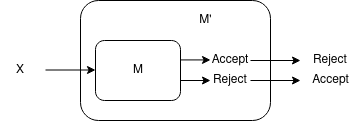
\includegraphics[width=0.6\textwidth]{/home/pedro/Carrera/Quinto/TFG/tesis/figures/Turing.png}
  \end{center}
  \caption{Turing Machine showcased in the proof.}
\end{figure}
\begin{figure}[h]
  \begin{center}
    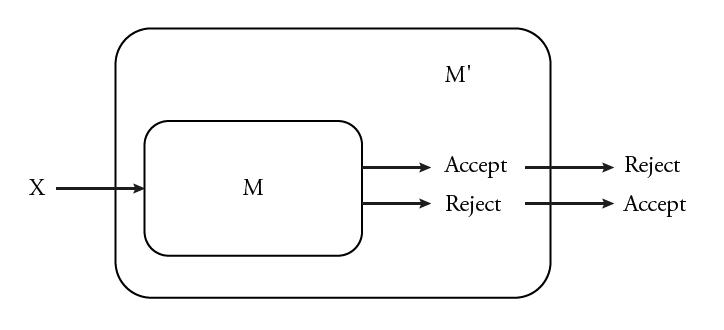
\includegraphics[width=0.6\textwidth]{/home/pedro/Carrera/Quinto/TFG/tesis/figures/Turing2.png}
  \end{center}
  \caption{Turing Machine showcased in the proof.}
\end{figure}


Nonetheless, this concept is really important for non-deterministic complexity classes, as the previous proposition is, in general, not known to be true. One of the most relevant open problems is whether or not CoNP = P. For us, CoNP is important also as is the class of TAUT.



\section{Completeness}

In this subsection we introduce the notion of completeness. This area was developed in late 1960s and early 1970s parallel by researchers on the US and the USSR, at during the Cold War. The first point in the development  of this theory and the most important result from the point of view of this text is the Cook-Levin theorem [\ref{ref:cooklevin}], which highlights the theoretical relevance of SAT. The notion of completeness was introduced to the Western World first by Cook \cite{cook1971complexity} although the term was coined later. \\

As a historical note, one of the first references to this notion is the Gödel's Letter\cite{hartmanis1993godel}, that he wrote to Von Neumann relating with the possibility of polynomially (in particular in linear or quadratic time) solving QBF (a generalization of SAT). He was asking, without knowing it, whether an NP-Complete problem could be solvable within polynomial time, and stating some of the consequences of this.\\



\subsection{Definition}

Once we have defined classes over the decision problems, and we have the concept of reduction, we want to use that in order to be able to solve whole classes only solving one of it problems.\\

Prior to that we have to revisit reductions. We have defined reductions without taking care of its complexity. Now we can fully define reductions

% \begin{definition}
%   Let $F,G$ be sets of endofunctions of $\mathbb{N}$:
%   \begin{enumerate}
%   \item  We say that a set of endofunctions $F$ of $\mathbb{N}$ is autocomposable if for every $f,g\in F$ there exists $h\in F$ such that $f\circ g \in O(h)$
%   \item We say that $F\le G$ if for every $f \in F, g \in G$ there exists $h\in G$ such that $g\circ f \in O(h)$. If $F$
%   \end{enumerate}
% \end{definition}


% We can see that the defined relationship over the set of autocomposable endofunctions is a preorder.
% \begin{proposition}
% P is autocomposable.
% \end{proposition}


\begin{definition}
  If $L_1$ and $L_2$ are decision problems.
\begin{enumerate}
\item We say that $L_1 \le_P L_2$ if there is an TM $M$ that always stops and computes a function $f$ such that for every $w \in L_1$ , we have that $f(w) \in L_2$, there is an $g\in P$ such that $M \in FTIME(g)$, and there is another $g'\in P$ such that $|f(w)| \in O(g(|w|))$.
\end{enumerate}
If $L_1 \le_{P} L_2$ we say that $L_1$ \emph{is reduced} to $L_2$.
\end{definition}




\begin{definition}
  Let $\Omega$ be a deterministic complexity class.  We say that a problem $L$ is $\Omega$\emph{-Complete} iff:
  \begin{itemize}
  \item $L \in\Omega.$
  \item For every $L' \in \Omega$, we have that $L' \le_P L$.
  \end{itemize}

If only the latter condition is satisfied, we say that $L$ is $\Omega$\emph{-Hard}.

\end{definition}


The set of P-Complete problems is the set of all problems that are reducible in polynomial time to a problem P and are in $P$. Now that we have defined both P-Completeness and NP-Completeness, we can continue our study. If one NP-Complete problem can be solve in Polynomial time, then P=NP. We have, nonetheless, a problem: How do we prove a problem to be NP-Complete? We have two ways:
\begin{enumerate}
\item To prove that every problem is reducible.
\item To reduce another NP-Complete problem in $P$.
\end{enumerate}

We can see that the latter option is preferable, as it involve less work. This option requires that one problem, at least, has been proven to be NP-Complete first, arguably with the first method. The next subsection deals with this matter, and reintroduces SAT as the main point of the text. 


\subsection{Cook-Levin Theorem}
At this point we introduce the main theorem of this section. The theorem was first sated on \cite{cook1971complexity}, although some ideas were first spoken about by Leonid Levin on 1969, the formal explanation of the result was first written by Stephen Cook. Due to our lack of knowledge of the Russian language we did not research Levin's original result, although we would like to point out that he did this research on the advice of the famous mathematician Kolmogorov. Also, later in his life, Levin emigrated to the US and was able to share his knowledge with the Western block\cite{cvlevincook}.\\




The theorem proves that SAT is NP-Complete, and was at the time the first completeness result provided. To this day virtually all proofs of problems to be NP-Complete are done by using either this result or using its ideas. For this theorem Cook received on 1982 the Turing Award, the highest honor conceded in the area of Computer Science. Without further ado with introduce the theorem, along with a brief lemma.\\

 Cook original result we can see that the modern standard statement of the theorem is an adaptation of the original statement done in theorem 1\\ \cite{cook1971complexity}. Instead of proving the result with the today-standard 3CNF satisfiability he proved the CoNP-Completeness result for TAUT, proving SAT NP-Completeness in the way. The proof showcased in this paper is the one followed to this dated by most text, with only a few adaptations. 

\begin{lemma}\label{lemma:cooklevin}
  For a set $A = \{a_1,...,a_n\}$ of Propositional Logic variables, we can define a set of clauses $\mathcal{C}(A)$ such that, for an assignment $alpha$ we have   $\mathcal{C}(A)\alpha = 1$ iff $\alpha$ maps to 1 one and only one of the variables in $A$.
\end{lemma}
\begin{proof}
  We define $$\mathcal{C}(A) = D\cup \left (  \cup_{i,j \in 1,..,n} D_{i,j} \right ),$$ where:
  \begin{equation}
    \begin{split}
      D & = (a_1 \vee ... \vee a_n ),\\
      D_{i,j} & = (\neg a_{i} \vee \neg a_{j} ).
\end{split}
\end{equation}

From $D$ it follows that $\alpha$ satisfy at least one variable, and from $D_{i,j}$ that $\alpha$ satisfy at most one.
\end{proof}


\begin{theorem}[Cook-Levin theorem]\label{ref:cooklevin}
 SAT is NP-Complete.
\end{theorem}
\begin{proof}
  Suppose that a language $L\subset A^*$ is accepted by a NDTM $M$ within time $O(q(n))$, where $q(n)$ is a polynomial. Given an input  $w\in A^*$ of $M$, we construct a CNF-Formula $\phi(w)$ such that $\phi(w)$ is satisfiable iff $M$ accepts $w$. As the construction is done in polynomial time, we have a polynomial reduction of the problem.
  
  Suppose that $\Gamma = \{\gamma_0,\gamma_1,...,\gamma_l\}$ is the tape alphabet  of $M$ with $B=\gamma_0$ .$Q=\{q_1,..,q_s\}$ is the set of states with $q_0$ the initial state. $\delta_0$ is the branching factor of $M$. $T(n)$\footnote{$M$ is in NP therefore $M$ is in PSPACE and as a consequence $T(n)$ exists } is the polynomial bound of the number of cells used by $M$. We define $T=T(|w|)$

  \begin{itemize}
  \item Firstly, we define the variables of $\phi(w)$.
    \begin{enumerate}
    \item The variables $\{p_{s,t}^i : 1 \le i \le l,\ 1 \le s,\ t \le T \}$. These variables represents (semantically) if tape cell $s$ at step $t$ contains the symbol $\gamma_i$.
    \item The variables $\{q_{t}^i : 1 \le i \le l,\ t \le T \}$ that represents if at step $t$ the machine is in state $q_i$.
    \item The variables $\{S_{s,t} :  1 \le s,\ t \le T \}$. These variables represents if tape cell $s$  is being scanned at step $t$.
    \item The variables $\{o_{d,t} :  1 \le d \le \delta_0,\ t \le T \}$. These variables represents that decision $d$ is made at step $t$.
    \end{enumerate}

  \item Once we have the variables, we define the clauses of $\phi(w)$.
    \begin{enumerate}
    \item For $t\le T$, the clauses $\mathcal{C}(S_t)$ with $S_t = \{S_{i,j}^t : i,j \le T\}$  that ensures that at time $t$ one and only one cell is being scanned.
    \item  For $t\le T$, the clauses $\mathcal{C}(C_{t})$ with $C_t = \{p_{s,t}^{i} : 1\le i \le l, 1 \le s \le T\}$ with  that ensures that one and only one symbol is at each step of the machine at each time.
    \item  For $t\le T$, the clauses $\mathcal{C}(O_{t})$ with $O_t = \{o_{d,t}^{i} : 1\le d \le \delta_0\}$ with  that ensures that one and only one decision is made at each step of the machine at each time.
    \item For $t\le T$, the clauses $\mathcal{C}(D_{t})$ with $D_t = \{q_t^{i} : 1\le i \le l\}$ with  that ensures that at time $t$ one and only one state is active.
    \item If $w = <\gamma_{i_1}...\gamma_{i_k}>$ we add the clauses $(p_{j,0}^{i_j})$ for $j$ in $1,...,k$. These clauses ensure the initial state. Also, for $j$ in $k+1,....,T$ we add $(p_{j,0}^0)$.  
    \item For each pair state-symbol $(q_k,\gamma_d)$ we let $\{(q_{k_1} , \gamma_{d_1} , m_1 ), ... , (q_{k_l} , \gamma_{d_l , m_l)} \subset Q \times \Gamma \times \{-1,1\}$ be the set of related transitions. We add the clauses:

    \[
    (\neg s_{s,t} \lor \neg q_t^i  \lor p_{s,t}^d \lor \neg o_{t, e}  \lor q_{t+1, k_e}),
    \]
    \[
(      \neg s_{s,t} \lor \neg q_t^i  \lor p_{s,t}^d \lor \neg o_{t, e}  \lor p_{s,t+1}^{d_e}),
    \]
    \[
(      \neg s_{s,t} \lor \neg q_t^i  \lor p_{s,t}^d \lor \neg o_{t, e}  \lor S_{s+m_e, t+1}),
    \]

    with $0 \le s,t \le T$, $0 \le d \le  \delta_0$. 

    If the set of related transitions is empty we add
    \[
    (\neg s_{s,t} \lor \neg q_t^i  \lor p_{s,t}^d \lor \neg o_{t, e}  \lor q_{t+1, k}),
    \]
    \[
(      \neg s_{s,t} \lor \neg q_t^i  \lor p_{s,t}^d \lor \neg o_{t, e}  \lor p_{s,t+1}^{d}),
    \]
    \[
(      \neg s_{s,t} \lor \neg q_t^i  \lor p_{s,t}^d \lor \neg o_{t, e}  \lor S_{s, t+1}),
    \]

    with $0 \le s,t \le T$, $0 \le d \le  \delta_0$.
    
    This represent the machine's operation.
  \item In order to maintain the tape unchanged in the cells where no operation is done we add:

    $$(\neg s_{t,s} \lor \neg p_{s,t}^i \lor  p_{s,t+1}^i),  $$
    for $0 \le s,t \le T$, $0 \le i \le l$.
  \item Suppose $\{q_{i_1},...,q_{i_k}\}$ is the set of final states. Then we add the clause:
    $$ (q_{i_1}^T \lor ... \lor q_{i_k}^T).$$

    That represents the necessity of the machine to end on a final state in order to accept $w$.
    \end{enumerate}


    The equivalence of the Problems is clear from the way the machine is built. The clauses reproduce exactly how the machine works for the entry word $w$ and include a clause that indicates that the word is accepted. If in the end (time $T$) the clause $ (q_{i_1}^T \lor ... \lor q_{i_k}^T)$ can be satisfied, then a state of acceptance can be reached. Then the word is accepted if and only if all are possible satisfy all the clauses.\\

As all operation described above can be done within polynomial time, we have found a P-reduction of any NP problem to SAT.
  \end{itemize}
\end{proof}


On the time of publication, this result was a truly breakthrough. On the technical part of the proof we would like to highlight the methods used, are they display two common cases that recurrently appears when reducing a problem to SAT.

\begin{itemize}
\item One and only one encodings, as the one showcased in the lemma, are common restriction for real-world problems. We decide to express this alternative in order to respect the original proof as much as possible, but also because this formulation is commonly believed to work better with DPLL based - solvers[\ref{sec:dpll}]. Different approaches to this reduction are considered in literature. For more information on this area we refer to subsection 2.2.4 \cite{darwiche2009complete}.

\item The rest of the clauses has at most one positive literal. These are the named Horn clauses. The particularity of this clauses resides in the fact that,
  $$(\neg u_1 \lor \neg u_2 ... \lor \neg u_n \lor v) \iff ((u_1\land ... \land u_n) \to v).$$
  That is, they are the natural language of implication in CNF. Because of theorem[\ref{theorem:hornsat}] we now that this language is enough to express polynomial DTM.
\end{itemize}





\subsection{Graph Isomorphism Problem}

In this subsection we introduce the Graph Isomorphism problem. We introduce this problem for two main reason:
\begin{itemize}
\item We want to make use of it in order to detect symmetries in CNF-Formulas.
\item It has a really interesting complexity class.
\end{itemize}

In this subsection we focus in the latter topic. In Subsection \ref{sub:Symmetry} we explain the interest of this problem in the context of SAT-solving. For more information on the problem we refer to \cite{fortin1996graph}. \\

In order to define a problem over graph, we have to be able to express them in a language. We can express any finite graph $G=(V,E)$ over an alphabet $\{0,..,9,B\}$:
\begin{enumerate}
\item We name each node in $V$ after number in $\mathbb{N}$, that is, we define an injective mapping $\phi: V \to \mathbb{N}$. Without any loss of generalization we can require this naming to be after the first $|V|$ naturals.
\item We start with the empty word $\epsilon$, and for every edge $(u,v)$\footnote{We consider $E\subset V\times V$.} concatenate at the end a word $\phi(u)B\phi(v)BB$.
\item When all edges are represented, concatenate at the end a word $BBB|V|$
\end{enumerate}

For example given:

\begin{figure}[H]
  \centering
  
  \begin{tikzpicture}[scale = 0.5,node distance=3cm,on grid,auto,thick] 
    % comentar para estilo básico
    \tikzstyle{every state}=[draw=myred!50,very thick,fill=myred!25,minimum size=1.2cm]
    \node[state] (q_0)   {$0$}; 
    \node[state] (q_1) [below=of q_0] {$1$}; 
    \node[state](q_2) [above right=of q_1] {$2$};
    \node[state](q_3) [above left=of q_1] {3};
    
    \path[->] 
    (q_1) edge node {} (q_0)
    (q_0) edge node {} (q_1)
    (q_1) edge node {} (q_2)
    (q_2) edge node {} (q_1)
    (q_3) edge node {} (q_1)
    (q_1) edge node {} (q_3)
    (q_2) edge node {} (q_0)
    (q_0) edge node {} (q_2);

    
  \end{tikzpicture}
  
  \caption{Example Graph}
\end{figure}

We can code it as $0B2BB2B0BB1B2BB2B1BB0B1BB1B0BB1B3BB3B1BBBBB4$. We name as \emph{GRAPH} to the language over $\{0,..,9,B\}$ that include all well formatted graphs. \\

\begin{definition}
  We define the Graph Isomorphism language ($GI$) as the subset $L\subset$ GRAPH $\times$ GRAPH such that for every pairs of words $(w_1,w_2)\in L$ theirs associated graphs are isomorphic. We name GI to the associated decision problem. \\
\end{definition}

Given a mapping between two graphs, it can be checked in polynomial time whether such mapping is an isomorphism. Therefore GI is in NP. GI is not known to be in P, neither to be NP-Complete. A complexity class is named after this problem:\\

\begin{definition}
  We define the class GI as the set of all decision problems that can be reduced to GI. \\
\end{definition}


Therefore a problem is GI complete if GI is reducible to it. As a historical note Las Vegas Algorithm is a probabilistic algorithm first introduced by László Babai in 1979 to solve this problem. 


\subsection{Other Completeness Results}

Although the most important completeness problems are the ones related with NP-Completeness, the concept of completeness can be implemented for every mayor complexity class. Most importantly for us, SAT variations are the norm for a lot of completeness results. On this subsection we will present the most important of these results.\\

The first result regards P-Completeness. 

\begin{theorem}[\cite{creignou1996complexity}]\label{theorem:hornsat}  HORNSAT is P-Complete
\end{theorem}

% TODO: Definir Circutitos o borrar este parrafo.
% To this day, the class P-complete is believed to be characterized by the problems that has to be computed sequentially. However, as many problems in this area, is still an open problem. The formal formulation of this problem is $$NC \myeq P$$ Where NC is Nick's class. This name was coined by Stephen Cook, in honor to Nick Pippenger and  is the class of decision problems solvable by a uniform family of Boolean circuits, with polynomial size, depth $O(log(n))$, and fan-in 2.\\

% Finding a parallelizable algorithm for HORNSAT would imply that $NC = P$. Nonetheless, it is widely believed that it is not possible. As being said, is still an open problem.\\



To continue,  we  present a brief discussion about FNP-Completeness. The same way we work with decision problems, we could be talking about Function Problem. In particular:


\begin{theorem} FSAT is FNP-Complete.  
\end{theorem}
To briefly sketch the proof, it  follows the one of the Cook-Levin theorem, only that we have the considerations of a function problem and therefore we have to state different final conditions.\\

The next problem we will discuss is QBF.

\begin{theorem}[\cite{franco2009history},theorem 4.11 \cite{arora2009computational}] QBF is PSPACE-Complete.
\end{theorem}

This in an important result as show the implicit difficult of automatically checking theorems in first order Logic. Nonetheless, it is worthy of considering, as the subsequent results of being able to solve this problem efficiently enough will make mathematicians life a lot easier, as theorem resolution will be a topic of well defined axioms and computer reasoning. This idea, was the one showcased in Gödel's Letter. \\

To end this subsection we will talk about CO-NP. We can use the study of NP Completeness in order to study CoNP Completeness.

\begin{proposition}
  Let $L$ be a language. $L$ is NP-Complete iff $CoL$ is CoNP-Complete.
\end{proposition}

\begin{proof}  \hfill
  \begin{itemize}
  \item[\fbox{$\Rightarrow$}] 
    Let $L'$ be a CoNP language. Therefore $CoL'$ is a NP language. There is a reduction $R$ from $CoL'$ to $L$ such that, $x \in CoL' \iff R(x) \in L$. Therefore $x \in L' \iff R(x) \in CoL$.
  \item[\fbox{$\Leftarrow$}] Analogue.
  \end{itemize}
\end{proof}

Therefore, UNSAT is CoNP complete and TAUT is CoNP complete.

\subsection{Exponential Time Hypothesis}
\label{hyp:exponential_time}
In this subsection we will introduce the hypothesis, shown first on \cite{impagliazzo2001complexity}. It states that no sub-exponential time algorithm can be found for 3-SAT. This hypothesis, although widely accepted, is still unproven. Formally:

\begin{definition}[ETH]
  For $k\ge 3$, lets define:
  $$s_k=\inf\{\delta: \text{there exists a } O(2^{\delta n})\ \ k-\text{ SAT solver}\}.$$
  It is claim that $s_k>0$.
\end{definition}

This result has some equivalent formulations.

\begin{proposition}[theorem 1. \cite{impagliazzo2001complexity}]
  The following statements are equivalent:
  \begin{enumerate}
  \item ETH: for all $k\ge 3$, $s_k > 0$.
  \item For some $k$, $s_k \ge 0$.
  \item $s_3 \ge 0$.

  \end{enumerate}
  \end{proposition}

This theorem is proven making use of The Sparsification Lemma, which is based in turn on the ideas of critical and forced variables. By the time of the publication of the article, Zane has already worked with these ideas for the development of the PPZ algorithm\cite{paturi1997satisfiability}. Although we are not going to prove this result, we are going to present this ideas when analyzing the Paturi-Pudlák-Zane Algorithm[\ref{subsec:PPZ}].
 
This claim is harder that $P\ne NP$, as it not only declares that SAT is not polynomial time, but neither is sub-exponential time. 







